% Compilar com pdfLaTeX (duas vezes), XeLaTeX ou LuaLaTeX.
% Manter a pasta assets ao lado deste arquivo. Exatamente 12 frames, sem overlays.
% Pacotes usados: tikz e tcolorbox (presentes no TeX Live, MiKTeX e Overleaf).
% Fontes científicas e procedência das imagens: LEIA-ME.md.
\PassOptionsToPackage{table}{xcolor}
\documentclass[aspectratio=169,11pt,t]{beamer}
\usepackage[utf8]{inputenc}
\usepackage[T1]{fontenc}
\IfFileExists{brazil.ldf}{\usepackage[brazil]{babel}}{\usepackage{babel}}
\usepackage{lmodern}
\usepackage{booktabs,array,graphicx,ragged2e}
\usepackage{tikz}
\usetikzlibrary{arrows.meta,positioning,calc}
\usepackage[most]{tcolorbox}

% ---------------------------------------------------------------- Paleta
\definecolor{navy}{HTML}{173545}
\definecolor{teal}{HTML}{087F78}
\definecolor{tealsoft}{HTML}{E4F1EE}
\definecolor{teallight}{HTML}{7FCFC4}
\definecolor{muted}{HTML}{5B6C77}
\definecolor{paper}{HTML}{FAFBF9}
\definecolor{line}{HTML}{D9E3DF}
\definecolor{amber}{HTML}{B4532A}
\definecolor{ambersoft}{HTML}{F8ECE4}

\setbeamercolor{background canvas}{bg=paper}
\setbeamercolor{normal text}{fg=navy,bg=paper}
\setbeamercolor{frametitle}{fg=navy}
\setbeamercolor{structure}{fg=teal}
\setbeamerfont{frametitle}{size=\Large,series=\bfseries}
\setbeamersize{text margin left=9mm,text margin right=9mm}
\setbeamertemplate{navigation symbols}{}
\setbeamertemplate{itemize item}{\color{teal}\small\textbullet}
\setlength{\parskip}{2pt}
\setbeamertemplate{frame begin}{\RaggedRight}
\hypersetup{colorlinks=true,urlcolor=teal,linkcolor=navy,
  pdftitle={Classificação de tumores cerebrais por transferência de aprendizado},
  pdfauthor={Pedro Brassi Luccas}}

% ---------------------------------------------------------------- Título com seção
\def\kickertext{}
\newcommand{\kicker}[1]{\gdef\kickertext{#1}}
\setbeamertemplate{frametitle}{%
  \vspace*{3.5mm}%
  \ifx\kickertext\empty\else
    {\fontsize{7.5}{9}\selectfont\bfseries\color{teal}%
     \rule[0.55ex]{5mm}{0.7pt}\enspace\kickertext\par}\vspace{0.4mm}%
  \fi
  {\usebeamerfont{frametitle}\color{navy}\insertframetitle\par}%
  \vspace{0.8mm}}

% ---------------------------------------------------------------- Rodapé com progresso
\setbeamertemplate{footline}{%
  \hspace{9mm}{\fontsize{7}{8}\selectfont\color{muted}Pedro Brassi Luccas\enspace·\enspace Projeto de TCC\enspace·\enspace UNIFAL-MG}%
  \hfill
  \begin{tikzpicture}[baseline=-0.4mm]
    \foreach \i in {1,...,12}{%
      \ifnum\i>\value{framenumber}\def\segcolor{line}\else\def\segcolor{teal}\fi
      \fill[\segcolor] ({(\i-1)*2.6mm},0) rectangle ++(2.1mm,0.8mm);}
  \end{tikzpicture}%
  \hspace{2.5mm}{\fontsize{7}{8}\selectfont\bfseries\color{muted}\insertframenumber\,/\,12}\hspace{9mm}%
  \par\vspace{3.5mm}}

% ---------------------------------------------------------------- Componentes
\tcbset{
  base/.style={enhanced,boxrule=0.5pt,arc=1.6mm,left=2.8mm,right=2.8mm,
    top=2mm,bottom=2mm,boxsep=0pt,fontupper=\small\color{navy},before upper=\RaggedRight},
  card/.style={base,colback=white,colframe=line},
  tint/.style={base,colback=tealsoft,colframe=tealsoft,left=4mm,
    overlay={\begin{tcbclipframe}\fill[teal] (frame.south west) rectangle ([xshift=1.2mm]frame.north west);\end{tcbclipframe}}},
  warn/.style={base,colback=ambersoft,colframe=ambersoft,left=4mm,
    overlay={\begin{tcbclipframe}\fill[amber] (frame.south west) rectangle ([xshift=1.2mm]frame.north west);\end{tcbclipframe}}},
  topstripe/.style={overlay={\begin{tcbclipframe}\fill[#1] (frame.north west) rectangle ([yshift=-1.1mm]frame.north east);\end{tcbclipframe}},top=3mm},
  banner/.style={base,colback=navy,colframe=navy,fontupper=\footnotesize\bfseries\color{white},top=2.2mm,bottom=2.2mm,left=4mm},
}
\newcommand{\labeltext}[1]{{\color{teal}\bfseries #1}\par}
\newcommand{\cardtitle}[2][teal]{{\color{#1}\bfseries #2}\par\vspace{0.5mm}}
\newcommand{\source}[1]{\par\vfill{\fontsize{6.5}{7.8}\selectfont\color{muted}#1\par}\vspace{1mm}}
\newcommand{\num}[2][teal]{\tikz[baseline=(n.base)]\node[circle,fill=#1,text=white,inner sep=0pt,minimum size=5.2mm,font=\scriptsize\bfseries](n){#2};}
\newcommand{\chipC}{\tikz[baseline=-0.65ex]\node[fill=teal,text=white,rounded corners=0.8mm,inner sep=0pt,minimum width=6.5mm,minimum height=3.4mm,font=\tiny\bfseries]{C};}
\newcommand{\chipP}{\tikz[baseline=-0.65ex]\node[fill=tealsoft,draw=teal,line width=0.5pt,text=teal,rounded corners=0.8mm,inner sep=0pt,minimum width=6.5mm,minimum height=3.4mm,font=\tiny\bfseries]{P};}
\newcommand{\chipE}{\tikz[baseline=-0.65ex]\node[draw=line,dashed,rounded corners=0.8mm,inner sep=0pt,minimum width=6.5mm,minimum height=3.4mm]{};}
\newcommand{\refitem}[3]{\textbf{#1}\par #2\par{\color{teal}#3}\par\vspace{0.9mm}}
% Imagem quadrada com fundo preto (preserva proporção, sem recorte)
\newcommand{\mri}[2]{\tikz\node[fill=black,inner sep=0pt,minimum width=#1,minimum height=#1]{\includegraphics[width=#1,height=#1,keepaspectratio]{#2}};}

\begin{document}

% ================================================================ 1. Capa
{\setbeamertemplate{background}{%
  \begin{tikzpicture}
    \useasboundingbox (0,0) rectangle (\paperwidth,\paperheight);
    \fill[paper] (0,0) rectangle (\paperwidth,\paperheight);
    \fill[navy] (106mm,0) rectangle (\paperwidth,\paperheight);
    \foreach \img/\lab/\x/\y in {glioma/Glioma/111/72, meningioma/Meningioma/134/72,
                                 hipofisario/Hipofisário/111/43, sem-tumor/Sem tumor/134/43}{%
      \node[anchor=north west,inner sep=0pt] at (\x mm,\y mm) {\mri{21mm}{assets/\img.jpg}};
      \node[anchor=north west,inner sep=0pt,text=teallight,font=\fontsize{6.5}{7}\selectfont\bfseries]
        at (\x mm,\y mm-22.2mm) {\lab};}
    \node[anchor=south west,inner sep=0pt,text=white!70!navy,font=\fontsize{5.5}{6.5}\selectfont,align=left]
      at (111mm,6mm) {Exemplos da base Brain Tumor MRI Dataset\\(Nickparvar, 2021). Rótulos da base.};
  \end{tikzpicture}}
\begin{frame}[plain]
\begin{minipage}[t][84mm][t]{88mm}\RaggedRight
\vspace{7mm}
{\fontsize{7.5}{9}\selectfont\bfseries\color{teal}\rule[0.55ex]{5mm}{0.7pt}\enspace UNIVERSIDADE FEDERAL DE ALFENAS\enspace·\enspace UNIFAL-MG\par}
\vspace{5mm}
{\fontsize{19}{22.5}\selectfont\bfseries\color{navy}Classificação de tumores cerebrais em imagens de ressonância magnética utilizando transferência de aprendizado\par}
\vspace{3mm}
{\small\color{muted}Uma análise comparativa de desempenho, eficiência computacional e explicabilidade\par}
\vfill
{\color{teal}\rule{12mm}{1.2pt}\par}
\vspace{2mm}
{\normalsize\bfseries Pedro Brassi Luccas\par}
{\small Orientador: Prof. Dr. Luiz Eduardo da Silva\par}
\vspace{3mm}
{\scriptsize\color{muted}TCC I\enspace·\enspace Ciência da Computação\enspace·\enspace 2026\par}
\vspace{2mm}
\end{minipage}
\end{frame}
}

% ================================================================ 2. Contextualização
\kicker{01\enspace CONTEXTO}
\begin{frame}{Contextualização}
\vspace{1mm}
\begin{columns}[T,onlytextwidth]
\column{.34\textwidth}
\centering
\mri{40mm}{assets/meningioma-contexto.jpg}\par
\vspace{1mm}
{\scriptsize\color{muted}Exemplo da classe ``meningioma''\par}
\column{.62\textwidth}
\vspace{2mm}
\renewcommand{\arraystretch}{1}
\begin{tabular}{@{}m{7mm}@{}>{\RaggedRight\arraybackslash}m{.88\linewidth}@{}}
\num{1} & A ressonância magnética permite visualizar detalhadamente estruturas cerebrais.\\[5mm]
\num{2} & A interpretação dos exames exige conhecimento especializado.\\[5mm]
\num{3} & A Inteligência Artificial pode auxiliar na identificação de padrões em imagens médicas.\\
\end{tabular}
\vspace{5mm}
\begin{tcolorbox}[tint]
\bfseries Como a computação pode contribuir para a análise dessas imagens?
\end{tcolorbox}
\end{columns}
\source{Imagem: Nickparvar (2021), Training/meningioma/Tr-me\_10.jpg. Rótulo fornecido pela base, sem validação clínica independente.}
\end{frame}

% ================================================================ 3. Literatura
\kicker{02\enspace PROBLEMA}
\begin{frame}{Resultados na literatura}
\relax
{\small Estudos recentes relatam acurácias elevadas na classificação de tumores cerebrais por IA.\par}
\vspace{1.5mm}
\begin{tcbraster}[raster columns=3,raster equal height,raster column skip=3.5mm]
\begin{tcolorbox}[card,topstripe=teal]
{\scriptsize\bfseries\color{muted}Disci et al. (2025)\par}\vspace{1mm}
{\fontsize{22}{24}\selectfont\bfseries\color{teal}98,73\%\par}\vspace{0.8mm}
{\footnotesize Acurácia ponderada, Xception\par}
\end{tcolorbox}
\begin{tcolorbox}[card,topstripe=teal]
{\scriptsize\bfseries\color{muted}Rasa et al. (2024)\par}\vspace{1.5mm}
{\fontsize{22}{24}\selectfont\bfseries\color{teal}99,96\%\par}\vspace{0.8mm}
{\footnotesize Validação cruzada em conjuntos menores\par}
{\scriptsize\color{muted}Conjuntos maiores: \mbox{96,34--98,20\%}\par}
\end{tcolorbox}
\begin{tcolorbox}[card,topstripe=teal]
{\scriptsize\bfseries\color{muted}Prayogo et al. (2025)\par}\vspace{1.5mm}
{\fontsize{22}{24}\selectfont\bfseries\color{teal}98,75\%\par}\vspace{0.8mm}
{\footnotesize Acurácia do modelo híbrido de CNNs\par}
\end{tcolorbox}
\end{tcbraster}
\vspace{1mm}
\begin{tcolorbox}[tint]
{\normalsize\bfseries Mas podemos confiar apenas nesses números?\par}
\vspace{0.5mm}
Uma acurácia elevada não garante, isoladamente, uma boa capacidade de generalização.
\end{tcolorbox}
\source{Metodologias e protocolos diferentes: valores não diretamente comparáveis.\enspace Disci et al.: 10.3390/cancers17010121.\enspace Rasa et al.: 10.1177/20552076241286140.\enspace Prayogo et al.: 10.1109/ACCESS.2025.3584376.}
\end{frame}

% ================================================================ 4. Vazamento e lacuna
% Não atribuir os achados de Yagis a tumores ou a qualquer estudo do slide 3.
\begin{frame}{Vazamento de dados: por que isso importa?}
\vspace{0.5mm}
\begin{columns}[T,onlytextwidth]
\column{.46\textwidth}
\begin{tcolorbox}[warn]
{\scriptsize\bfseries\color{amber}Yagis et al. (2021)\par}
{\fontsize{24}{27}\selectfont\bfseries\color{amber}Até 55 p.p.\par}
\vspace{0.5mm}
{\footnotesize de inflação artificial da acurácia com divisão inadequada em fatias 2D, em bases de Alzheimer e Parkinson.\par}
\end{tcolorbox}
\vspace{1.5mm}
\begin{tcolorbox}[card]
{\scriptsize\bfseries\color{teal}Fateh et al. (2026)\par}
\vspace{0.5mm}
{\footnotesize Removeram duplicatas exatas e quase duplicatas \textbf{antes da divisão}, em uma base derivada do mesmo conjunto público.\par}
\end{tcolorbox}
\column{.50\textwidth}
\centering
\begin{tikzpicture}[font=\scriptsize]
  \node[draw=line,fill=white,rounded corners=1.5mm,inner sep=1.6mm] (tr) {\mri{15mm}{assets/exemplo-vazamento.jpg}};
  \node[draw=amber,line width=0.8pt,fill=white,rounded corners=1.5mm,inner sep=1.6mm,right=15mm of tr] (te) {\mri{15mm}{assets/exemplo-vazamento.jpg}};
  \node[above=0.6mm of tr,font=\scriptsize\bfseries,text=navy] {Treinamento};
  \node[above=0.6mm of te,font=\scriptsize\bfseries,text=amber] {Teste};
  \node[below=0.4mm of tr,font=\tiny,text=muted] {Imagem A};
  \node[below=0.4mm of te,font=\tiny,text=muted] {Cópia da imagem A};
  \draw[{Stealth[length=2mm]}-{Stealth[length=2mm]},amber,thick,dashed] (tr.east) -- node[above=0.5mm,align=center,text=amber,font=\tiny\bfseries]{mesma\\imagem} (te.west);
\end{tikzpicture}\par
\vspace{0.2mm}
{\fontsize{6.5}{7.8}\selectfont\color{muted}Esquema conceitual com repetição intencional: o teste deixa de ser independente.\par}
\vspace{1.5mm}
\raggedright
\begin{tcolorbox}[tint]
{\scriptsize\bfseries\color{teal}Lacuna investigada\par}
\vspace{0.5mm}
{\footnotesize Auditoria da base original combinada à comparação entre ResNet50, EfficientNet-B0 e MobileNetV3.\par}
\end{tcolorbox}
\end{columns}
\source{Yagis et al. (2021); Fateh et al. (2026). Imagem: Nickparvar (2021), Tr-gl\_10.jpg. Lacuna conforme levantamento preliminar.}
\end{frame}

% ================================================================ 5. Objetivos
\kicker{03\enspace PROPOSTA}
\begin{frame}{Objetivos da pesquisa}
\vspace{0.5mm}
\begin{tcolorbox}[tint,fontupper=\footnotesize\color{navy}]
{\scriptsize\bfseries\color{teal}OBJETIVO GERAL\par}
\vspace{0.6mm}
Desenvolver e avaliar modelos de classificação de tumores cerebrais em imagens de ressonância magnética utilizando transferência de aprendizado, considerando desempenho, eficiência computacional, deduplicação e explicabilidade.
\end{tcolorbox}
\vspace{2mm}
{\scriptsize\bfseries\color{teal}OBJETIVOS ESPECÍFICOS\par}
\vspace{0.8mm}
\begin{tcbraster}[raster columns=4,raster equal height,raster column skip=3mm]
\begin{tcolorbox}[card,top=1.6mm,bottom=1.6mm,left=2.2mm,right=2.2mm,fontupper=\footnotesize\color{navy}]
{\fontsize{13}{15}\selectfont\bfseries\color{teal}01\par}\vspace{0.4mm}
\textbf{Auditar a base}\par\vspace{0.4mm}
Analisar as imagens e identificar duplicatas exatas ou visualmente semelhantes.
\end{tcolorbox}
\begin{tcolorbox}[card,top=1.6mm,bottom=1.6mm,left=2.2mm,right=2.2mm,fontupper=\footnotesize\color{navy}]
{\fontsize{13}{15}\selectfont\bfseries\color{teal}02\par}\vspace{0.4mm}
\textbf{Treinar os modelos}\par\vspace{0.4mm}
Aplicar uma CNN simples e três arquiteturas pré-treinadas.
\end{tcolorbox}
\begin{tcolorbox}[card,top=1.6mm,bottom=1.6mm,left=2.2mm,right=2.2mm,fontupper=\footnotesize\color{navy}]
{\fontsize{13}{15}\selectfont\bfseries\color{teal}03\par}\vspace{0.4mm}
\textbf{Comparar os resultados}\par\vspace{0.4mm}
Avaliar desempenho, custo computacional e efeito da deduplicação.
\end{tcolorbox}
\begin{tcolorbox}[card,top=1.6mm,bottom=1.6mm,left=2.2mm,right=2.2mm,fontupper=\footnotesize\color{navy}]
{\fontsize{13}{15}\selectfont\bfseries\color{teal}04\par}\vspace{0.4mm}
\textbf{Investigar as decisões}\par\vspace{0.4mm}
Analisar os erros e explorar as regiões destacadas pelo Grad-CAM.
\end{tcolorbox}
\end{tcbraster}
\end{frame}

% ================================================================ 6. Base e preparação
\kicker{04\enspace METODOLOGIA}
\begin{frame}{Base de dados e preparação}
\relax
{\small\textbf{Brain Tumor MRI Dataset} (Nickparvar, 2021), disponível no Kaggle: quatro categorias\par}
\vspace{1.5mm}
\begin{columns}[T,onlytextwidth]
\column{.24\textwidth}\centering\mri{14mm}{assets/glioma.jpg}\par{\scriptsize\bfseries Glioma}
\column{.24\textwidth}\centering\mri{14mm}{assets/meningioma.jpg}\par{\scriptsize\bfseries Meningioma}
\column{.24\textwidth}\centering\mri{14mm}{assets/hipofisario.jpg}\par{\scriptsize\bfseries Tumor hipofisário}
\column{.24\textwidth}\centering\mri{14mm}{assets/sem-tumor.jpg}\par{\scriptsize\bfseries Ausência de tumor}
\end{columns}
\vspace{3mm}
\centering
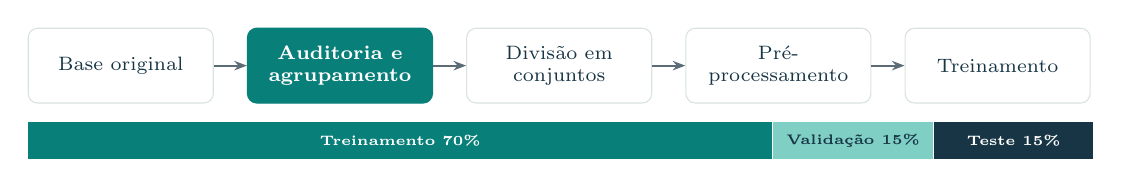
\begin{tikzpicture}[
  stage/.style={draw=line,fill=white,rounded corners=1.2mm,text width=21.5mm,minimum height=9.5mm,align=center,font=\scriptsize,text=navy,inner sep=1mm},
  key/.style={stage,fill=teal,draw=teal,text=white,font=\scriptsize\bfseries},
  arr/.style={-{Stealth[length=1.6mm]},muted,thick}]
  \node[stage] (a) {Base original};
  \node[key,right=4.2mm of a] (b) {Auditoria e agrupamento};
  \node[stage,right=4.2mm of b] (c) {Divisão em conjuntos};
  \node[stage,right=4.2mm of c] (d) {Pré-processamento};
  \node[stage,right=4.2mm of d] (e) {Treinamento};
  \foreach \u/\v in {a/b,b/c,c/d,d/e} \draw[arr] (\u) -- (\v);
  % Barra de divisão 70/15/15
  \coordinate (L) at ($(a.west)+(0,-9.5mm)$);
  \coordinate (R) at ($(e.east)+(0,-9.5mm)$);
  \path let \p1=(L), \p2=(R), \n1={\x2-\x1} in
    node[fill=teal,text=white,font=\tiny\bfseries,minimum height=4.6mm,minimum width={0.70*\n1},inner sep=0,anchor=west] (t1) at (L) {Treinamento 70\%}
    node[fill=teallight,text=navy,font=\tiny\bfseries,minimum height=4.6mm,minimum width={0.15*\n1},inner sep=0,anchor=west] (t2) at (t1.east) {Validação 15\%}
    node[fill=navy,text=white,font=\tiny\bfseries,minimum height=4.6mm,minimum width={0.15*\n1},inner sep=0,anchor=west] (t3) at (t2.east) {Teste 15\%};
\end{tikzpicture}\par
\vspace{2mm}
\raggedright
{\footnotesize Duplicatas identificadas agrupadas no mesmo conjunto\enspace\textcolor{teal}{\textbullet}\enspace Redimensionamento e normalização\enspace\textcolor{teal}{\textbullet}\enspace Aumento de dados somente no treino\par}
\source{Fonte: Nickparvar (2021). Rótulos da base. Sem identificadores para garantir separação por paciente.}
\end{frame}

% ================================================================ 7. Modelos e experimentos
% Sete experimentos centrais, conforme páginas 6 e 7 do pré-projeto.
\begin{frame}{Modelos e plano experimental}
\vspace{0.5mm}
\begin{columns}[T,onlytextwidth]
\column{.40\textwidth}
\labeltext{\scriptsize ARQUITETURAS PRÉ-TREINADAS}
\vspace{0.6mm}
\begin{tcolorbox}[card,top=1.6mm,bottom=1.6mm,fontupper=\footnotesize\color{navy}]
\textbf{ResNet50}\par{\scriptsize\color{muted}Rede profunda com conexões residuais\par}
\vspace{0.8mm}{\color{line}\hrule}\vspace{1mm}
\textbf{EfficientNet-B0}\par{\scriptsize\color{muted}Equilíbrio entre desempenho e eficiência\par}
\vspace{0.8mm}{\color{line}\hrule}\vspace{1mm}
\textbf{MobileNetV3}\par{\scriptsize\color{muted}Arquitetura compacta e eficiente\par}
\end{tcolorbox}
\vspace{1.5mm}
\begin{tcolorbox}[tint,top=1.6mm,bottom=1.6mm,fontupper=\footnotesize\color{navy}]
\textbf{Transferência de aprendizado}\par
{\scriptsize Aproveitamento de características aprendidas previamente para adaptar os modelos à classificação de ressonâncias magnéticas.\par}
\end{tcolorbox}
\column{.56\textwidth}
\labeltext{\scriptsize PLANO EXPERIMENTAL}
\vspace{0.6mm}
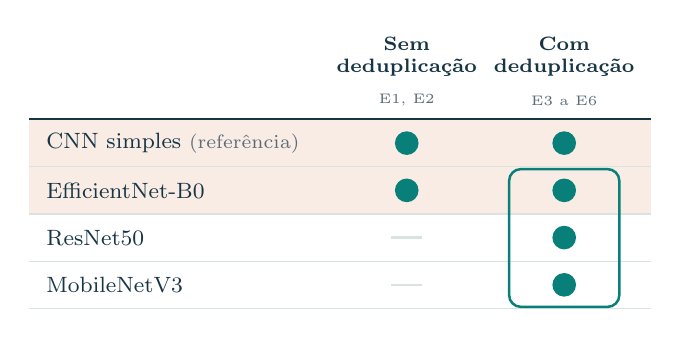
\begin{tikzpicture}[font=\footnotesize,x=1mm,y=1mm]
  % faixas
  \def\rowh{6}
  \fill[ambersoft] (0,3) rectangle (79,-9);
  \foreach \r/\name in {0/CNN simples {\color{muted}\scriptsize(referência)},1/EfficientNet-B0,2/ResNet50,3/MobileNetV3}{
    \node[anchor=west,text=navy] at (1,{-\r*\rowh}) {\name};
    \draw[line] (0,{-\r*\rowh-3}) -- (79,{-\r*\rowh-3});}
  % cabeçalho
  \node[font=\scriptsize\bfseries,align=center,text=navy] at (48,11) {Sem\\deduplicação};
  \node[font=\scriptsize\bfseries,align=center,text=navy] at (68,11) {Com\\deduplicação};
  \node[font=\tiny,text=muted] at (48,5.4) {E1, E2};
  \node[font=\tiny,text=muted] at (68,5.4) {E3 a E6};
  \draw[navy,thick] (0,3.1) -- (79,3.1);
  % destaque coluna deduplicada (arquiteturas)
  \draw[teal,line width=0.9pt,rounded corners=1.5mm] (61,-3.3) rectangle (75,-20.8);
  % marcadores
  \foreach \x/\y in {48/0,48/-6,68/0,68/-6,68/-12,68/-18}{\fill[teal] (\x,\y) circle (1.5);}
  \foreach \y in {-12,-18}{\draw[line,thick] (46,\y) -- (50,\y);}
\end{tikzpicture}\par
\vspace{1.2mm}
{\scriptsize
\tikz[baseline=-0.6ex]\fill[ambersoft] (0,-1mm) rectangle (4mm,1.2mm);\enspace\textbf{Efeito da deduplicação:} CNN simples e EfficientNet-B0\par
\vspace{0.4mm}
\tikz[baseline=-0.6ex]\draw[teal,line width=0.9pt,rounded corners=0.6mm] (0,-1mm) rectangle (4mm,1.2mm);\enspace\textbf{Comparação das arquiteturas:} na base deduplicada\par}
\vspace{1.6mm}
\begin{tcolorbox}[tint,top=1.4mm,bottom=1.4mm,fontupper=\footnotesize\color{navy}]
\textbf{E7:} análise de erros e explicabilidade com Grad-CAM no modelo selecionado.
\end{tcolorbox}
\end{columns}
\end{frame}

% ================================================================ 8. Avaliação
% Definição precisa de Macro F1; Grad-CAM conceitual, sem mapa simulado.
\begin{frame}{Avaliação dos modelos e explicabilidade}
\vspace{0.5mm}
\begin{tcolorbox}[card,topstripe=teal,fontupper=\footnotesize\color{navy}]
\cardtitle{Desempenho de classificação}
\renewcommand{\arraystretch}{1.12}
\begin{tabular}{@{}>{\RaggedRight\arraybackslash}p{.47\linewidth}@{\hspace{.05\linewidth}}>{\RaggedRight\arraybackslash}p{.47\linewidth}@{}}
\textbf{Acurácia:} proporção de acertos & \textbf{Matriz de confusão:} identificação dos erros\\
\textbf{Macro F1:} média dos F1 das quatro classes, com igual peso & \textbf{AUC-ROC:} capacidade de discriminação, uma classe contra as demais\\
\end{tabular}
\end{tcolorbox}
\vspace{2mm}
\nointerlineskip
\noindent\begin{minipage}[t]{.38\textwidth}\vspace{0pt}
\begin{tcolorbox}[card,topstripe=navy,height=19mm,fontupper=\footnotesize\color{navy}]
\cardtitle[navy]{Eficiência computacional}
Número de parâmetros\par Tamanho do modelo (MB)\par Tempo de inferência
\end{tcolorbox}
\end{minipage}\hfill
\begin{minipage}[t]{.595\textwidth}\vspace{0pt}
\begin{tcolorbox}[card,topstripe=amber,height=19mm,fontupper=\footnotesize\color{navy}]
\cardtitle[amber]{Explicabilidade: Grad-CAM}
Regiões que contribuíram para a pontuação do modelo.\par
Análise exploratória do melhor modelo, em acertos e erros.
\end{tcolorbox}
\end{minipage}\par
\vspace{2mm}
\begin{tcolorbox}[banner]
Avaliar quanto o modelo acerta, quanto custa e quais regiões influenciam suas decisões.
\end{tcolorbox}
\source{Selvaraju et al. (2017). Grad-CAM não é segmentação nem comprovação de correção clínica.}
\end{frame}

% ================================================================ 9. Resultados esperados e limitações
\kicker{05\enspace PERSPECTIVAS}
\begin{frame}{Resultados esperados e limitações}
\vspace{0.5mm}
\begin{tcbraster}[raster columns=2,raster equal height,raster column skip=4mm]
\begin{tcolorbox}[card,topstripe=teal,fontupper=\footnotesize\color{navy}]
\cardtitle{Resultados esperados}
\textbf{Impacto da deduplicação}\par
Investigar se a remoção de duplicatas modifica as métricas de classificação.\par\vspace{0.7mm}
\textbf{Comparação das arquiteturas}\par
Identificar diferenças entre desempenho e custo computacional.\par\vspace{0.7mm}
\textbf{Análise das decisões}\par
Explorar erros e regiões destacadas pelo Grad-CAM.
\end{tcolorbox}
\begin{tcolorbox}[card,topstripe=amber,fontupper=\footnotesize\color{navy}]
\cardtitle[amber]{Limitações}
\textbf{Identificação dos pacientes}\par
A base não disponibiliza identificadores para garantir separação por paciente.\par\vspace{0.7mm}
\textbf{Generalização}\par
Resultados em uma base pública não garantem desempenho em outros contextos.\par\vspace{0.7mm}
\textbf{Aplicação clínica}\par
O projeto não pretende validar uma ferramenta de diagnóstico médico.
\end{tcolorbox}
\end{tcbraster}
\vspace{1.5mm}
\begin{tcolorbox}[tint,top=1.6mm,bottom=1.6mm]
\textbf{Contribuição esperada:} uma avaliação mais criteriosa da classificação de tumores cerebrais por Inteligência Artificial.
\end{tcolorbox}
\end{frame}

% ================================================================ 10. Cronograma
% Reprodução da tabela visível da página 8 do pré-projeto. Células vazias são intencionais.
\begin{frame}{Cronograma da pesquisa}
\relax
{\small Planejamento indicativo de seis meses, a ajustar com o orientador\par}
\vspace{0.5mm}
\centering
{\fontsize{8.3}{9.2}\selectfont
\renewcommand{\arraystretch}{1.0}
\setlength{\tabcolsep}{4pt}
\rowcolors{2}{white}{tealsoft!55}
\begin{tabular}{@{}>{\raggedright\arraybackslash}p{62mm}*{6}{>{\centering\arraybackslash}p{10.5mm}}@{}}
\toprule
\rowcolor{paper}\textbf{Atividade} & \textbf{Mês 1}&\textbf{Mês 2}&\textbf{Mês 3}&\textbf{Mês 4}&\textbf{Mês 5}&\textbf{Mês 6}\\
\midrule
Tema e problema & \chipC &&&&&\\
Revisão bibliográfica & \chipP &&&&&\\
Base e documentação & \chipC &&&&&\\
Auditoria/deduplicação &&&&&&\\
Pré-processamento &&&&&&\\
Baseline &&&&&&\\
Treinamento (E1--E6) &&&&&&\\
Ajustes &&&&&&\\
Avaliação &&&&&&\\
Grad-CAM (E7) &&&&&&\\
Extensões (se houver tempo) &&&&&&\\
Redação & \chipP &&&&&\\
Revisão/apresentação &&&&&&\\
\bottomrule
\end{tabular}\par}
\raggedright
\par\vfill
{\scriptsize\color{muted}\chipC\,concluído\quad\chipP\,parcialmente realizado\quad vazio: período a definir\hfill Fonte: pré-projeto, p. 8\par}\vspace{1mm}
\end{frame}

% ================================================================ 11. Considerações finais
{\setbeamertemplate{background}{%
  
\begin{tikzpicture}
    \useasboundingbox (0,0) rectangle (\paperwidth,\paperheight);
    \fill[navy] (0,0) rectangle (\paperwidth,\paperheight);
    \fill[teal] (0,0) rectangle (\paperwidth,1.2mm);
  \end{tikzpicture}}
\begin{frame}[plain]
\begin{minipage}[t][84mm][t]{\textwidth}\RaggedRight
\vspace{9mm}
{\fontsize{7.5}{9}\selectfont\bfseries\color{teallight}\rule[0.55ex]{5mm}{0.7pt}\enspace CONSIDERAÇÕES FINAIS\par}
\vspace{5mm}
{\fontsize{22}{27}\selectfont\bfseries\color{white}Mais do que obter uma alta acurácia, é necessário avaliar a \textcolor{teallight}{confiabilidade} dos resultados.\par}
\vspace{7mm}

\begin{tikzpicture}[pill/.style={draw=teallight,text=white,rounded corners=3.2mm,minimum height=6.4mm,inner xsep=4mm,font=\small}]
  \node[pill] (p1) {Qualidade dos dados};
  \node[pill,right=3mm of p1] (p2) {Avaliação comparativa};
  \node[pill,right=3mm of p2] {Explicabilidade};
\end{tikzpicture}\par
\vfill
{\fontsize{20}{24}\selectfont\bfseries\color{white}Obrigado!}\enspace{\large\color{teallight}Perguntas?}\par
\vspace{2mm}
{\small\color{white!70!navy}Pedro Brassi Luccas\enspace·\enspace Ciência da Computação\enspace·\enspace UNIFAL-MG\hfill 11\,/\,12\par}
\vspace{5mm}
\end{minipage}
\end{frame}
}

% ================================================================ 12. Referências
\kicker{}
\begin{frame}{Referências bibliográficas}
\fontsize{6.7}{7.8}\selectfont
\setlength{\parskip}{0pt}
\begin{columns}[T,onlytextwidth]
\column{.49\textwidth}
\labeltext{Classificação e qualidade dos dados}
\vspace{0.8mm}
\refitem{DISCI, R.; GURCAN, F.; SOYLU, A. (2025)}{Advanced brain tumor classification in MR images using transfer learning and pre-trained deep CNN models. \textit{Cancers}, 17, 121.}{\href{https://doi.org/10.3390/cancers17010121}{DOI: 10.3390/cancers17010121}}
\refitem{RASA, S. M. et al. (2024)}{Brain tumor classification using fine-tuned transfer learning models on magnetic resonance imaging (MRI) images. \textit{Digital Health}, 10.}{\href{https://doi.org/10.1177/20552076241286140}{DOI: 10.1177/20552076241286140}}
\refitem{PRAYOGO, R. D.; HAMID, N.; NAMBO, H. (2025)}{Hybrid CNN-Based Transfer Learning Enhances Brain Tumor Classification on MRI Images. \textit{IEEE Access}, 13, 116654--116668.}{\href{https://doi.org/10.1109/ACCESS.2025.3584376}{DOI: 10.1109/ACCESS.2025.3584376}}
\refitem{YAGIS, E. et al. (2021)}{Effect of data leakage in brain MRI classification using 2D convolutional neural networks. \textit{Scientific Reports}, 11, 22544.}{\href{https://doi.org/10.1038/s41598-021-01681-w}{DOI: 10.1038/s41598-021-01681-w}}
\refitem{FATEH, A. et al. (2026)}{BRISC: Annotated Dataset for Brain Tumor Segmentation and Classification. \textit{Scientific Data}, 13, 361.}{\href{https://doi.org/10.1038/s41597-026-06753-y}{DOI: 10.1038/s41597-026-06753-y}}
\column{.47\textwidth}
\labeltext{Base, arquiteturas e explicabilidade}
\vspace{0.8mm}
\refitem{NICKPARVAR, M. (2021)}{Brain Tumor MRI Dataset. Kaggle.}{\href{https://www.kaggle.com/datasets/masoudnickparvar/brain-tumor-mri-dataset}{kaggle.com/datasets/masoudnickparvar/brain-tumor-mri-dataset}}
\refitem{HE, K. et al. (2016)}{Deep Residual Learning for Image Recognition. \textit{CVPR}, p. 770--778.}{\href{https://doi.org/10.1109/CVPR.2016.90}{DOI: 10.1109/CVPR.2016.90}}
\refitem{TAN, M.; LE, Q. V. (2019)}{EfficientNet: Rethinking Model Scaling for Convolutional Neural Networks. \textit{PMLR}, 97, p. 6105--6114.}{\href{https://proceedings.mlr.press/v97/tan19a.html}{proceedings.mlr.press/v97/tan19a.html}}
\refitem{HOWARD, A. et al. (2019)}{Searching for MobileNetV3. \textit{ICCV}, p. 1314--1324.}{\href{https://doi.org/10.1109/ICCV.2019.00140}{DOI: 10.1109/ICCV.2019.00140}}
\refitem{SELVARAJU, R. R. et al. (2017)}{Grad-CAM: Visual Explanations from Deep Networks via Gradient-Based Localization. \textit{ICCV}, p. 618--626.}{\href{https://doi.org/10.1109/ICCV.2017.74}{DOI: 10.1109/ICCV.2017.74}}
\end{columns}
\end{frame}

\end{document}
